% Options for packages loaded elsewhere
\PassOptionsToPackage{unicode}{hyperref}
\PassOptionsToPackage{hyphens}{url}
%
\documentclass[
  man]{apa6}
\usepackage{amsmath,amssymb}
\usepackage{lmodern}
\usepackage{iftex}
\ifPDFTeX
  \usepackage[T1]{fontenc}
  \usepackage[utf8]{inputenc}
  \usepackage{textcomp} % provide euro and other symbols
\else % if luatex or xetex
  \usepackage{unicode-math}
  \defaultfontfeatures{Scale=MatchLowercase}
  \defaultfontfeatures[\rmfamily]{Ligatures=TeX,Scale=1}
\fi
% Use upquote if available, for straight quotes in verbatim environments
\IfFileExists{upquote.sty}{\usepackage{upquote}}{}
\IfFileExists{microtype.sty}{% use microtype if available
  \usepackage[]{microtype}
  \UseMicrotypeSet[protrusion]{basicmath} % disable protrusion for tt fonts
}{}
\makeatletter
\@ifundefined{KOMAClassName}{% if non-KOMA class
  \IfFileExists{parskip.sty}{%
    \usepackage{parskip}
  }{% else
    \setlength{\parindent}{0pt}
    \setlength{\parskip}{6pt plus 2pt minus 1pt}}
}{% if KOMA class
  \KOMAoptions{parskip=half}}
\makeatother
\usepackage{xcolor}
\usepackage{graphicx}
\makeatletter
\def\maxwidth{\ifdim\Gin@nat@width>\linewidth\linewidth\else\Gin@nat@width\fi}
\def\maxheight{\ifdim\Gin@nat@height>\textheight\textheight\else\Gin@nat@height\fi}
\makeatother
% Scale images if necessary, so that they will not overflow the page
% margins by default, and it is still possible to overwrite the defaults
% using explicit options in \includegraphics[width, height, ...]{}
\setkeys{Gin}{width=\maxwidth,height=\maxheight,keepaspectratio}
% Set default figure placement to htbp
\makeatletter
\def\fps@figure{htbp}
\makeatother
\setlength{\emergencystretch}{3em} % prevent overfull lines
\providecommand{\tightlist}{%
  \setlength{\itemsep}{0pt}\setlength{\parskip}{0pt}}
\setcounter{secnumdepth}{-\maxdimen} % remove section numbering
% Make \paragraph and \subparagraph free-standing
\ifx\paragraph\undefined\else
  \let\oldparagraph\paragraph
  \renewcommand{\paragraph}[1]{\oldparagraph{#1}\mbox{}}
\fi
\ifx\subparagraph\undefined\else
  \let\oldsubparagraph\subparagraph
  \renewcommand{\subparagraph}[1]{\oldsubparagraph{#1}\mbox{}}
\fi
\newlength{\cslhangindent}
\setlength{\cslhangindent}{1.5em}
\newlength{\csllabelwidth}
\setlength{\csllabelwidth}{3em}
\newlength{\cslentryspacingunit} % times entry-spacing
\setlength{\cslentryspacingunit}{\parskip}
\newenvironment{CSLReferences}[2] % #1 hanging-ident, #2 entry spacing
 {% don't indent paragraphs
  \setlength{\parindent}{0pt}
  % turn on hanging indent if param 1 is 1
  \ifodd #1
  \let\oldpar\par
  \def\par{\hangindent=\cslhangindent\oldpar}
  \fi
  % set entry spacing
  \setlength{\parskip}{#2\cslentryspacingunit}
 }%
 {}
\usepackage{calc}
\newcommand{\CSLBlock}[1]{#1\hfill\break}
\newcommand{\CSLLeftMargin}[1]{\parbox[t]{\csllabelwidth}{#1}}
\newcommand{\CSLRightInline}[1]{\parbox[t]{\linewidth - \csllabelwidth}{#1}\break}
\newcommand{\CSLIndent}[1]{\hspace{\cslhangindent}#1}
\ifLuaTeX
\usepackage[bidi=basic]{babel}
\else
\usepackage[bidi=default]{babel}
\fi
\babelprovide[main,import]{english}
% get rid of language-specific shorthands (see #6817):
\let\LanguageShortHands\languageshorthands
\def\languageshorthands#1{}
% Manuscript styling
\usepackage{upgreek}
\captionsetup{font=singlespacing,justification=justified}

% Table formatting
\usepackage{longtable}
\usepackage{lscape}
% \usepackage[counterclockwise]{rotating}   % Landscape page setup for large tables
\usepackage{multirow}		% Table styling
\usepackage{tabularx}		% Control Column width
\usepackage[flushleft]{threeparttable}	% Allows for three part tables with a specified notes section
\usepackage{threeparttablex}            % Lets threeparttable work with longtable

% Create new environments so endfloat can handle them
% \newenvironment{ltable}
%   {\begin{landscape}\centering\begin{threeparttable}}
%   {\end{threeparttable}\end{landscape}}
\newenvironment{lltable}{\begin{landscape}\centering\begin{ThreePartTable}}{\end{ThreePartTable}\end{landscape}}

% Enables adjusting longtable caption width to table width
% Solution found at http://golatex.de/longtable-mit-caption-so-breit-wie-die-tabelle-t15767.html
\makeatletter
\newcommand\LastLTentrywidth{1em}
\newlength\longtablewidth
\setlength{\longtablewidth}{1in}
\newcommand{\getlongtablewidth}{\begingroup \ifcsname LT@\roman{LT@tables}\endcsname \global\longtablewidth=0pt \renewcommand{\LT@entry}[2]{\global\advance\longtablewidth by ##2\relax\gdef\LastLTentrywidth{##2}}\@nameuse{LT@\roman{LT@tables}} \fi \endgroup}

% \setlength{\parindent}{0.5in}
% \setlength{\parskip}{0pt plus 0pt minus 0pt}

% Overwrite redefinition of paragraph and subparagraph by the default LaTeX template
% See https://github.com/crsh/papaja/issues/292
\makeatletter
\renewcommand{\paragraph}{\@startsection{paragraph}{4}{\parindent}%
  {0\baselineskip \@plus 0.2ex \@minus 0.2ex}%
  {-1em}%
  {\normalfont\normalsize\bfseries\itshape\typesectitle}}

\renewcommand{\subparagraph}[1]{\@startsection{subparagraph}{5}{1em}%
  {0\baselineskip \@plus 0.2ex \@minus 0.2ex}%
  {-\z@\relax}%
  {\normalfont\normalsize\itshape\hspace{\parindent}{#1}\textit{\addperi}}{\relax}}
\makeatother

% \usepackage{etoolbox}
\makeatletter
\patchcmd{\HyOrg@maketitle}
  {\section{\normalfont\normalsize\abstractname}}
  {\section*{\normalfont\normalsize\abstractname}}
  {}{\typeout{Failed to patch abstract.}}
\patchcmd{\HyOrg@maketitle}
  {\section{\protect\normalfont{\@title}}}
  {\section*{\protect\normalfont{\@title}}}
  {}{\typeout{Failed to patch title.}}
\makeatother

\usepackage{xpatch}
\makeatletter
\xapptocmd\appendix
  {\xapptocmd\section
    {\addcontentsline{toc}{section}{\appendixname\ifoneappendix\else~\theappendix\fi\\: #1}}
    {}{\InnerPatchFailed}%
  }
{}{\PatchFailed}
\keywords{O*Net, challenge-hindrance framework, job demands-resoures, job characteristics\newline\indent Word count: X}
\DeclareDelayedFloatFlavor{ThreePartTable}{table}
\DeclareDelayedFloatFlavor{lltable}{table}
\DeclareDelayedFloatFlavor*{longtable}{table}
\makeatletter
\renewcommand{\efloat@iwrite}[1]{\immediate\expandafter\protected@write\csname efloat@post#1\endcsname{}}
\makeatother
\usepackage{lineno}

\linenumbers
\usepackage{csquotes}
\ifLuaTeX
  \usepackage{selnolig}  % disable illegal ligatures
\fi
\IfFileExists{bookmark.sty}{\usepackage{bookmark}}{\usepackage{hyperref}}
\IfFileExists{xurl.sty}{\usepackage{xurl}}{} % add URL line breaks if available
\urlstyle{same} % disable monospaced font for URLs
\hypersetup{
  pdftitle={Job Demands-Resources Model Components through the Lens of O*NET Classifications},
  pdfauthor={Alicia Stachowski1, John Kulas2, \& Renata Garcia Prieto Palacios Roji3},
  pdflang={en-EN},
  pdfkeywords={O*Net, challenge-hindrance framework, job demands-resoures, job characteristics},
  hidelinks,
  pdfcreator={LaTeX via pandoc}}

\title{Job Demands-Resources Model Components through the Lens of O*NET Classifications}
\author{Alicia Stachowski\textsuperscript{1}, John Kulas\textsuperscript{2}, \& Renata Garcia Prieto Palacios Roji\textsuperscript{3}}
\date{}


\shorttitle{O*NET JD-R}

\authornote{

Funding: This work was supported by the College of Humanities and Social Sciences, Montclair State University, Montclair, NJ.

Correspondence concerning this article should be addressed to Alicia Stachowski, 470M Harvey Hall, 721 3rd Street E, Menomenie, WI, 54751, USA. E-mail: \href{mailto:stachowskia@uwstout.edu}{\nolinkurl{stachowskia@uwstout.edu}}

}

\affiliation{\vspace{0.5cm}\textsuperscript{1} University of Wisconsin-Stout\\\textsuperscript{2} eRg\\\textsuperscript{3} PepsiCo}

\abstract{%
Much of our understanding of job demands and resources rests on the assumption that some aspects and components of one's job are resources and some are demands. We build on a small but growing literature suggesting that individual differences may matter in our perceptions of characteristics as demands and resources. The primary aims were to explore 1) whether there is variability in subjective ratings of job characteristics with respect to how much they served as resources and demands, and 2) whether or not there was a match between the literature-implicated resources/demands and subjective ratings of these characteristics. O*NET work characteristics were rated by 568 employed respondents in terms of relevance, perception as a demand, and perception as a resource. The results suggest that job characteristics differ in variability/stability regarding subjective worker perceptions, particularly for hindrance demands which showed the most variability. Job characteristics were not uniquely categorized as a resource or demand, and literature-implicated resources were also implicated as being challenge, but not hindrance demands.
}



\begin{document}
\maketitle

Research on the job demands-resources model (Demerouti et al., 2001) and later job demands-resources theory (Bakker \& Demerouti, 2017) highlights the importance of work characteristics on the experience of motivation and strain, which subsequently have an impact on job performance, among other outcomes. However, much of our existing knowledge regarding the way this model functions is grounded in the assumption that job characteristics are generally considered resources or generally considered demands. We build on the work of a small, but growing number of researchers who argue that the characteristics of work may be appraised simultaneously as resources and demands (Webster et al., 2011) or that appraisals may change over time (Rosen et al., 2020). We extend this critical research to that of the subjective distinction between challenge and hindrance demands (and resources) in the workplace, with a primary aims of exploring 1) whether there is variability in subjective ratings of job characteristics with respect to how much they serve as resources and demands, and 2) whether or not there is a match between the literature-implicated resources/demands and subjective ratings of these characteristics. Prior to presenting the current study in detail, we provide a brief overview of the relevant theories and relevant empirical work on this topic.

\hypertarget{the-job-demands-resources-theory}{%
\subsection{The Job demands-Resources Theory}\label{the-job-demands-resources-theory}}

The overarching context for this study is that of the job demands-resources theory, which is an expansion of the well-studied job demands-resources model (Demerouti et al., 2001). One of the major advantages of the job demands-resources theory is that it allows us to model both work environment and job characteristics via job resources and demands. \emph{Resources} include physical, psychological, social, or organizational aspects of the job that may help an employee achieve work goals, reduce job demands, or promote personal growth and development (Demerouti et al., 2001). In contrast, demands include components of a job that require sustained effort, and as such, produce psychological or physiological strain {[}e.g., high work pressure is frequently cited as a common demand; Demerouti et al. (2001){]}. Cognitively, the perception of an element of one's job as a resource or demand activates one of two distinct processes: either health impairment (resulting from demands) or motivation {[}resulting from resources; Bakker and Demerouti (2014){]}. Of particular importance here is that it is the perception of a characteristic or situation determines which process an employee will experience despite the typical \emph{a priori} assignment of a characteristic as objectively a ``demand'' or ``resource''. We explore this further below.

\hypertarget{the-essential-role-of-appraisal}{%
\subsection{The Essential Role of Appraisal}\label{the-essential-role-of-appraisal}}

As described above, job context and characteristics are assigned or appraised as demands or resources. Although much of our research on job demands in particular is based on \emph{a priori} classifications (Searle \& Auton, 2015), the classification of a work characteristic as a demand or resource is largely subjective by nature (e.g., an employee could most certainly perceive being a public figure as a resource or as a demand). The stress process speaks to how such individual difference in appraisal is possible. Lazarus and Folkman (1984) presented the transactional theory of stress and coping, which states that people cognitively appraise stimuli in their environments on a continuous basis. Via this process, meaning is assigned to stimuli based on potential for gain or loss. If appraised as threatening, challenging, or possibly harmful, the resulting emotional distress initiates coping. The cycle of appraisal then continues based on the action to cope with the stressor (Lazarus \& Folkman, 1984). Coping is considered a secondary appraisal and is the way that someone chooses to manage a stressor. Although not suggested by the names, primary and secondary appraisals can happen simultaneously. For instance, available resources to cope with a stressor may influence an employee's initial appraisal of a stressor (e.g., amount of time {[}resource{]} available to prepare for the speech may influence one's primary appraisal of this task).

\hypertarget{the-challenge-hindrance-stressor-framework}{%
\subsection{The Challenge-hindrance Stressor Framework}\label{the-challenge-hindrance-stressor-framework}}

Although there is a tendency to attach a negative connotation to the word ``stress'', Selye (1936) defined stress as simple a response to change. We return to the public figure for this next section. Consider two employees be called upon to serve as spokespeople for their organization. One may appraise the circumstance as an opportunity to positively influence others, while the other may feel daunted by the task.

The challenge-hindrance stressor framework suggests that the way we understand reactions to stressors requires consideration of how people feel about a given stressor (Cavanaugh et al., 2000), in line with Lazarus and Folkman (1984). Cavanaugh et al. (2000) delineated between two forms of demands -- that of \emph{challenge} and \emph{hindrance} demands. Challenge demands promote mastery, personal growth, and future gains -- these stressors should lead to coping strategies that facilitate achievement. Stressors like time pressure and responsibility are considered challenge stressors/demands. Hindrance demands, in contrast, inhibit growth, learning and goal achievement. Hindrance stressors (e.g., role conflict, role ambiguity, politics) are associated with negative job behaviors and attitudes. This distinction between challenges and hindrances has been of value in determining which demands are related to various outcomes. The original work on this topic suggests that challenge stressors are typically associated with positive outcomes and hindrance stressors are associated with negative outcomes (e.g., Cavanaugh et al., 2000).

Prior to considering the subsequent empirical work on this topic, it is of value to explore \emph{why} different outcomes are expected with these forms of demands. M. A. LePine (2022) explain the mechanisms by which demands are related to performance and wellbeing outcomes. Similar to the job-demands resources theory (Bakker \& Demerouti, 2017), challenge and hindrance demands elicit two different paths or processes. First, challenge stressors typically result in a challenge appraisal, and engagement is likely to happen as a result. Engagement, in turn, is positively related to motivation, performance, growth, and wellbeing. Of note is that this energy may be depleted eventually, leading to strain. Hindrance stressors elicit a different process. Disengagement is likely to result from a hindrance appraisal, which in contrast, negatively impacts motivation, performance, growth and wellbeing. This happens because resources are depleted via frustrations and other affectively negative reactions (M. A. LePine, 2022).

We next consider the empirical evidence on this topic. The first question we should ask is whether people distinguish between challenge vs.~hindrance demands, or whether all demands are under a larger ``demands'' category. Evidence suggests the employees do, in fact, differentiate between challenge and hindrance stressors (e.g., Bakker \& Sanz-Vergel, 2013; Gerich, 2017; Webster et al., 2011). For example, Bakker and Sanz-Vergel (2013) found that work pressure was perceived as a hindrance demand, and emotional demands as more of a challenge demand. Webster et al. (2011) approached this question with three common workplace demands: workload, role ambiguity, and role conflict. They found while that each could be appraised primarily as a challenge or hindrance demand, they could also simultaneously be perceived as being both a challenge and hindrance demand to different degrees.

Appraisals are associated with different forms of coping, and subsequently, outcomes. The challenge-hindrance stressor framework has been associated with a wide variety of organizational outcomes ranging from affective variables like job satisfaction, to motivation, performance, and wellbeing. A sampling of variables and relationships are described below to provide a sense of scope of the work that has been on this topic. Kim and Beehr (2020) found that appraising a demand (in their study, workload, responsibility, and learning demands were measured) as a challenge was associated with motivational resources (i.e., sense of self-worth and work meaningfulness), which were positively related to flourishing. The opposite occurred when a demand was appraised as a hindrance -- in those instances, the appraisal had a negative association with motivational resources. Cavanaugh et al. (2000), in a study of managers, found that challenge demands were positively related to job satisfaction and negatively related to job search behaviors, while hindrance demands demonstrated the opposite pattern. Chen et al. (2021) found that daily challenge demands were positively related to cognitive wellbeing and work-family enrichment. Daily hindrance demands were negatively related to these outcomes. In contrast, Abbas and Raja (2019) found that challenge and hindrance stressors were \emph{both} positively related to strain and turnover intentions. We also have some evidence that challenge-hindrance appraisals are related to engagement in the expected direction whereby hindrance appraisals are negatively associated with engagement and challenge appraisals are positively associated with it (Crawford et al., 2010). Challenge and hindrance appraisals have also been shown to relate to citizenship and counterproductive performance, although indirectly via emotions like anxiety (Rodell \& Judge, 2009). Lastly, Gerich (2017) concluded that employee wellbeing was also, in part, explained by appraised challenge or hindrance demands such that working conditions of time pressure, qualitative demands, responsibility, and interruptions, were partially mediated by challenge and hindrance demands.

We even have sufficient evidence to explore outcomes associated with challenge and hindrance stressors meta-analytically at this point, and a rich collection of them support differential associations across a variety of organizational outcomes as well. For example, both challenges and hindrances have been shown to positively predict strain (J. A. LePine et al., 2005; Podsakoff et al., 2007; Webster et al., 2010). Many other outcomes are differentially related to challenges and hindrances, largely in the expected direction. For example, motivation, job satisfaction, commitment, and performance have been shown to positively relate to challenge stressors and negatively relate to hindrance stressors (J. A. LePine et al., 2005). Turnover intentions, turnover and withdrawal behaviors are negatively related to hindrance stressors (Podsakoff et al., 2007). Kim and Beehr (2020), similarly, found evidence for the differential results via challenge and hindrance appraisals.

Horan et al. (2020) and M. A. LePine (2022) specifically call out the need for additional research to incorporate the appraisal process described by Lazarus and Folkman (1984) into the challenge-hindrance stressor framework, which aligns with other calls to capture subjective ratings of demands and resources into our study of the overarching JD-R model. In fact, Horan et al. (2020) state that ``\ldots stressors are only challenge or hindrance stressors to the extent that they are perceived as such by employees'' (p.~3). They go on to suggest future research continue to move away from \emph{a priori} classifications of stressors, as doing so can be problematic for theoretical and empirical reasons. Theoretically, \emph{a priori} classifications run counter to the original transactional theory of stress on which the challenge-hindrance stressor framework was based for which appraisals are a central component. Empirically, as shown above, we have some evidence suggesting people can appraise a stressor as both a hindrance and challenge at the same time (e.g., Searle \& Auton, 2015).

\hypertarget{current-study-and-hypotheses}{%
\subsection{Current Study and Hypotheses}\label{current-study-and-hypotheses}}

The integration of the literature above culminates with two primary hypotheses. The first addresses whether employees generally agree on their appraisals of job characteristics as resources or challenge or hindrance demands. For instance, although challenge stressors tend to be appraised more so as challenges, and hindrance stressors tend to be appraised more as hindrances than challenges, others have reported variability in these appraisals (e.g., M. A. LePine, 2022). M. A. LePine (2022), in fact, argues that the challenge-hindrance stressor framework acknowledges that these appraisals are not universal. Thus, it is quite possible, given the theoretical and empirical evidence presented above, that there is wide variability in individual appraisal of work activities and context such that some people may rate a given activity as a resource and others a hindrance.

\begin{quote}
Hypothesis 1: Job characteristics differ in consistancy regarding subjective worker perception as a demand or resource.
\end{quote}

\begin{quote}
Hypothesis 2: Job characteristics are not exclusively categorized as a resource or demand, but rather, some job characteristics are viewed as both a resource and a demand.
\end{quote}

Two exploratory questions further address whether our \emph{literature-implicated} resources (e.g., autonomy) and demands are consistently rated as our research models suggest across the job-demands resources theory (Bakker \& Demerouti, 2017) and challenge-hindrance stressor framework (Cavanaugh et al., 2000).

\begin{quote}
\emph{Research Question 1}: Do literature-implicated resources materialize as perceived resources?
\end{quote}

\begin{quote}
\emph{Research Question 2}: Do literature-implicated demands materialize as job demands?
\end{quote}

\hypertarget{method}{%
\section{Method}\label{method}}

\hypertarget{participants}{%
\subsection{Participants}\label{participants}}

Of the 785 individuals who initially accessed the survey link, 112 indicated that they were not interested, had more than 200 missing responses, or had 20 or more identical consecutive sequential responses (Yentes \& Wilhelm, 2021). Applying a further screen regarding attention checks (there were four attention checks embedded throughout, asking respondents to indicate a specific answer) resulted in the retention of 568 respondents who constitute the current sample. Regarding tenure, 13.57\% had been in their referent job less than 6 months, 19.20\% between 6 months and a year, 49.12\% between one and five years, 13.27\% between 5 and 10 years, and 4.87\% more than 10 years. Respondent ages ranged from 18 to 65 with an average of 28.18 years old (\emph{SD} = 7.53). The survey offered a free-field gender identity category, although the sample predominantly self-identified as female (52.58\%) or male (46.83\%).

\hypertarget{materials}{%
\subsection{Materials}\label{materials}}

The Occupational Information Network (O*Net) contains a comprehensive description of occupations (Peterson et al., 2001). This widely accessed database houses hundreds of standardized and occupation-specific descriptors of occupations in the US and these descriptions are continually updated. We focused on 98 work \href{https://www.ONETonline.org/find/descriptor/result/4.A.1.b.3}{activity and context statements} which O*Net groups into \emph{activity} categories of information input (e.g., where and how are the information and data gained that are needed to perform this job?), interacting with others (e.g., what interactions with other persons or supervisory activities occur while performing this job?), mental processes (e.g., what processing, planning, problem-solving, decision-making, and innovating activities are performed with job-relevant information?) and work output (e.g., what physical activities are performed, what equipment and vehicles are operated/controlled, and what complex/technical activities are accomplished as job outputs?). Work \emph{context} statements are grouped into interpersonal relationships (e.g., the context of the job in terms of human interaction processes), physical work conditions (e.g., the work context as it relates to the interactions between the worker and the physical job environment), and structural job characteristics (e.g., the relationships or interactions between the worker and the structural characteristics of the job).

O*Net collects information about these categories by periodically asking workers job characteristic questions, which often have \href{https://www.ONETonline.org/find/descriptor/result/4.C.1.c.2}{unique response categories}. For example, ``How responsible is the worker for work outcomes and results of other workers?'' has response options ranging from \emph{no responsibility} to \emph{very high responsibility}, while the question, ``How often do you use electronic mail in this job?'' has options ranging from \emph{never} to \emph{every day}. We retained O*Net's response scales while asking for statement relevance, all of which shared the same 5-point scale regardless of semantic label difference. Other than minor grammatical editing (for example, changing ``the worker'' to ``you''), we also retained the O*Net wording for our item stems.

\hypertarget{procedure}{%
\subsection{Procedure}\label{procedure}}

Data were collected through Prolific, an online data collection platform. An email was sent to a random subset of all eligible participants in the Prolific respondent pool, notifying them about their eligibility for the study based on demographic information. Eligibility requirements included being 18 or older and holding either a full-time or part-time job. Participants then voluntarily chose to respond to the online survey. Participants were asked to think about their primary job, and the items they were presented with depended on the specific job characteristics they initially specified. Thus, if a respondent indicated that a characteristic was not part of their job, they were not subsequently asked to rate the level of resource (\ldots this aspect of your job is a resource that can be functional in achieving work goals, reduce job demands, or stimulate personal growth/development), challenge (\ldots this aspect of your job is a challenge that can promote mastery, personal growth, or future gains), or hindrance (\ldots this aspect of your job is a hindrance that can inhibit personal growth, learning, and work goal attainment) in randomized order. The total number of items on the survey was less than 392 (98 characteristics x 4 repeated measurements) because we did not ask for demand and resource evaluations for 14 O*Net characteristics that we projected would have very low frequency of endorsement across respondents (one excluded characteristic, for example, was \emph{\ldots the extent to which the worker is exposed to radiation on the job}). Participants were compensated for their participation in this study estimated to require 45 minutes' time in the amount of six dollars through Prolific.

\hypertarget{results}{%
\section{Results}\label{results}}

\begin{figure}
\centering
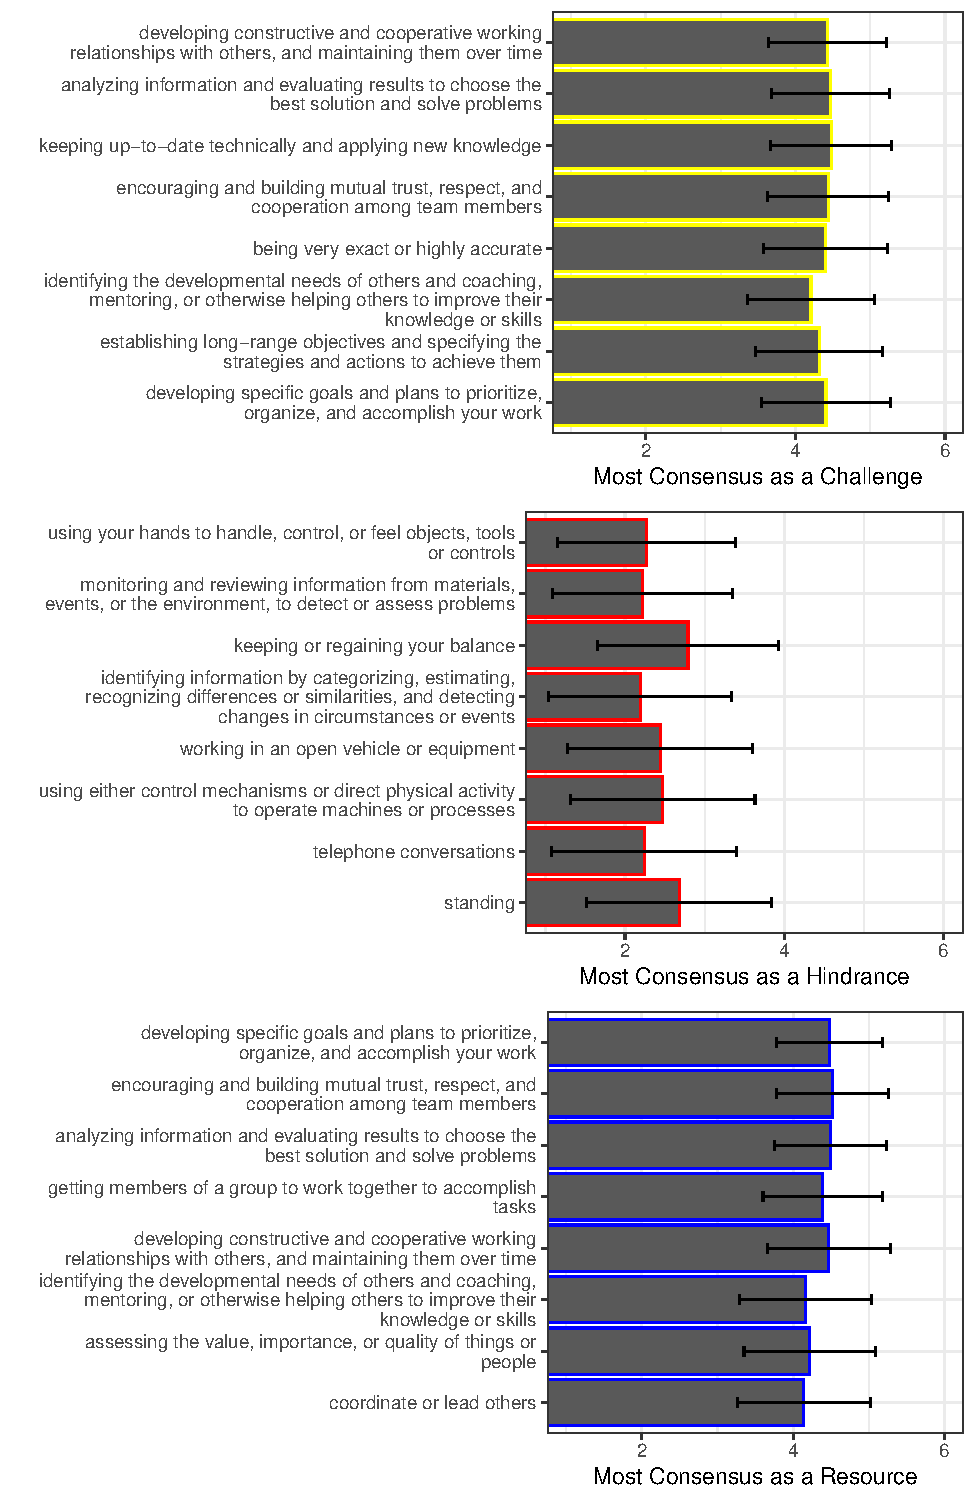
\includegraphics{Submission_files/figure-latex/combinegraphs-1.pdf}
\caption{\label{fig:combinegraphs}Characteristics percieved most similarly (lowest standard deviations).}
\end{figure}

\begin{figure}
\centering
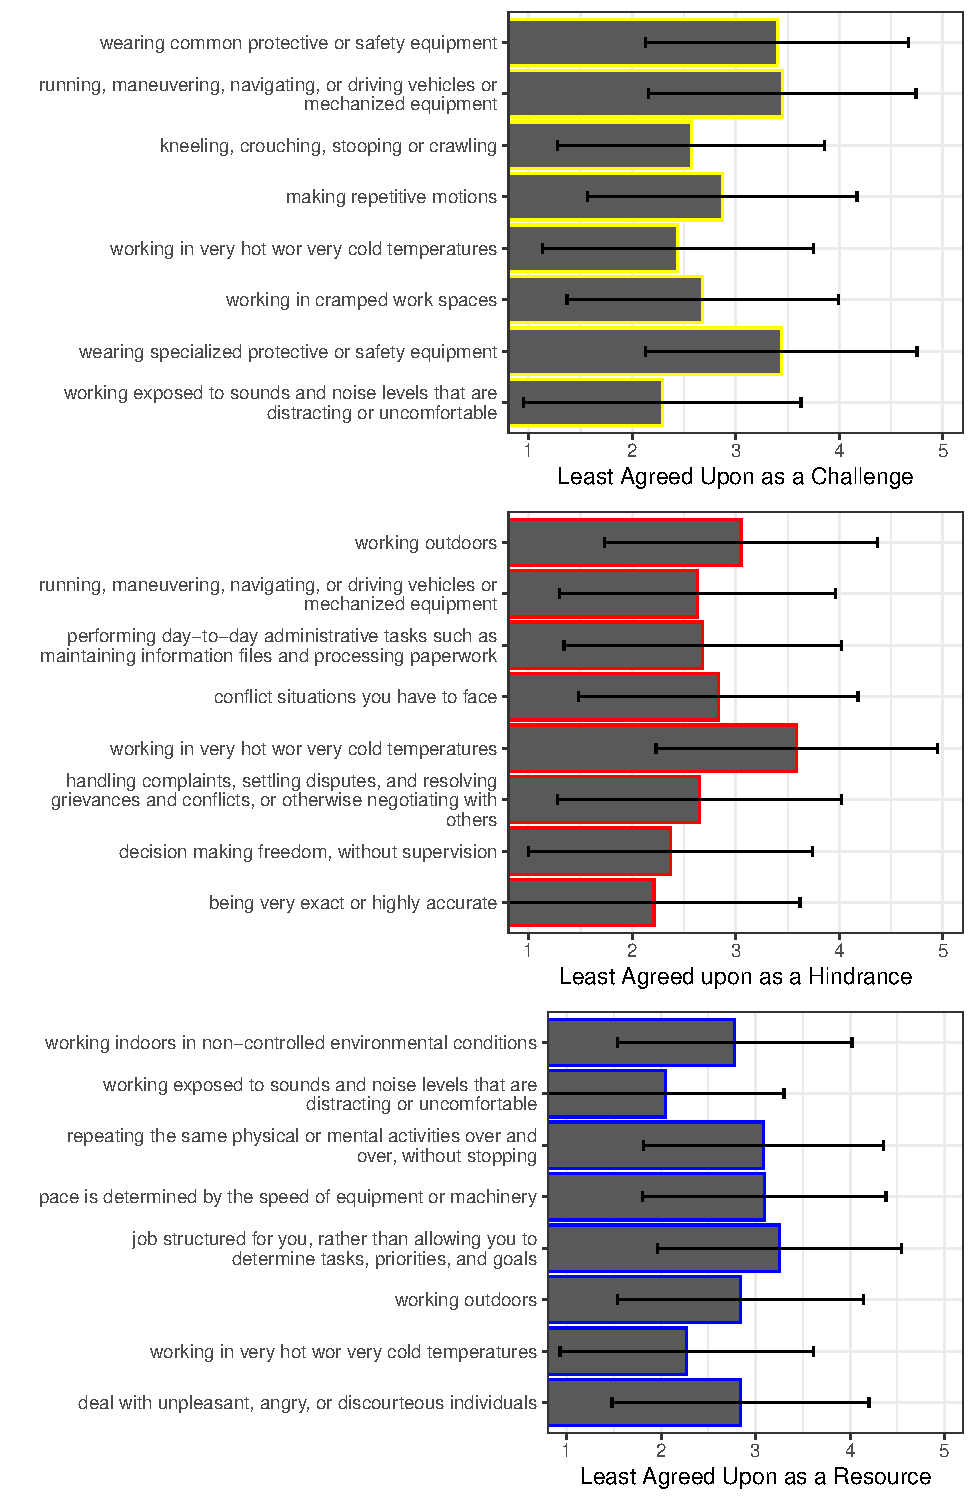
\includegraphics{Submission_files/figure-latex/combinegraphs2-1.pdf}
\caption{\label{fig:combinegraphs2}Characteristics percieved most \emph{DIS}similarly (largest standard deviations).}
\end{figure}

\begin{figure}
\centering
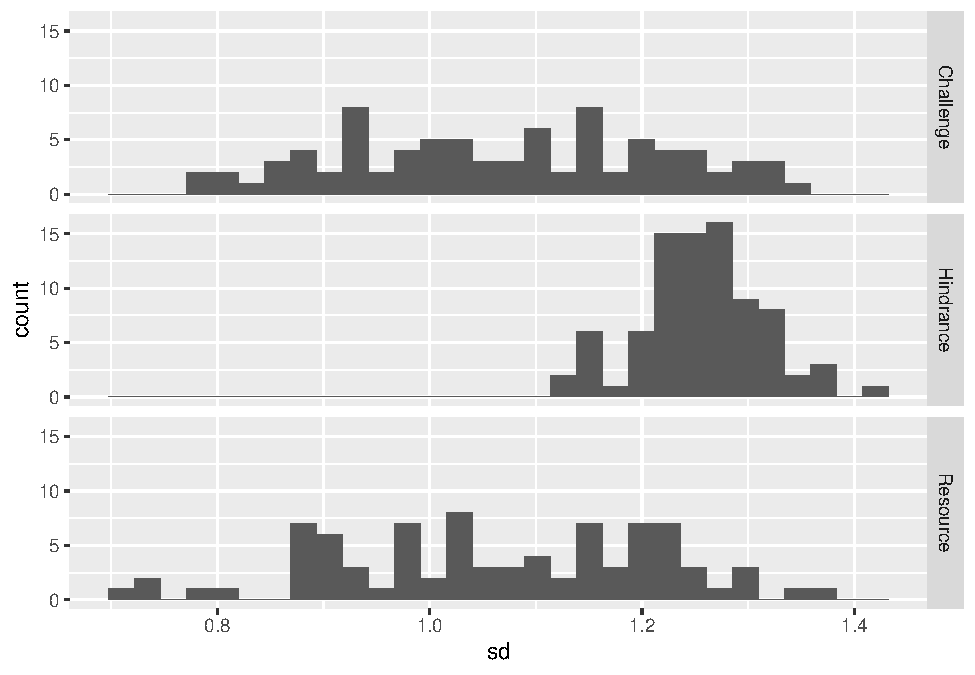
\includegraphics{Submission_files/figure-latex/overallhist-1.pdf}
\caption{\label{fig:overallhist}Frequency distribution of standard deviations across characteristics deemed resources, challenges, and demands.}
\end{figure}

H1 posits that static job characteristics are not necessarily always experienced similarly across workers - as hindrances, challenges, or resources. We explore this hypothesis first at the job characteristic level before presenting a broader perspective. Figures \ref{fig:combinegraphs} and \ref{fig:combinegraphs2} present only extreme snapshots of characteristic variability in the form of the 8-most \emph{consistently rated} and \emph{inconsistently rated} resources, challenges, and demands.\footnote{A full list of item characteristic ratings, along with summary averages and standard deviations is available in supplementary online resources. The Figures \ref{fig:combinegraphs} and \ref{fig:combinegraphs2} presentations are only limited to 8 characteristics per perceived category because of space restrictions (there are 252 individual characteristic ratings in the online resources).} These figures present average item ratings, but the central elements of interest are the standard deviations, which reflect the characteristics with the relative greatest and least consistency. Figure \ref{fig:combinegraphs} presents the resources, challenges, and hindrances that are \emph{most consistently agreed on} as indexed by (relatively) low standard deviations, while Figure \ref{fig:combinegraphs2} presents the characteristics with the greatest amount of \emph{disagreement} across workers. The figures demonstrate that what is widely seen as a resource and challenge tends to be somewhat agreed upon (the range of the ``lowest 8'' resource standard deviations is 0.70 to 0.88 and the range of lowest 8 challenge standard deviations is 0.79 to 0.86). However, there is considerably less relative agreement regarding the degree to which job elements should be considered to be hindrances, with the 8 elements showing the \emph{greatest agreement} still ranging in fairly large standard deviations (ranging from 1.12 to 1.16).

In addition to highlighting extremely agreed- or disagreed-upon items, Figure \ref{fig:overallhist} presents our standard deviation indices across all rated items. Here, the Figure \ref{fig:combinegraphs} discrepancies receive greater context, with the \emph{spread} of difference exhibiting wider distributions of agreement for challenge and resource ratings (and relatively \emph{bunched} levels of disagreement for hindrances; note the spread of the challenge and resource histograms relative to the hindrance histogram). Some characteristics are largely agreed upon as being challenges and resources, while all hindrance perceptions exhibit a relatively higher level of disagreement. This points to \emph{hindrances}, in particular, as being likely amenable to future probing regarding moderating conditions. A Bartlett's test for homogeneity of variance across the challenge, hindrance, and resource ratings confirms this difference (\(\chi^2_{}\) = 76.83, \emph{p} \textless{} .01). In sum, these results provide some collective support for H1, and particularly so for hindrances, which are differently experienced across our raters.

The second hypothesis stated that job characteristics would not be uniquely categorized as a resource or demand. Table \ref{tab:cortab} provides the correlations among the O*Net ``scale''-level groupings across ratings of resource, challenge, and hindrance. We would expect to see minimal correlations if job characteristics \emph{were} uniquely categorized. First, the average correlation within all resource categories (variables 1 through 7 in Table \ref{tab:cortab}) was .43 (\emph{SD} = .13, range from .15 to .64), and challenge categories exhibited similar associations (ranging from .12 to .70, \emph{M} = .43, \emph{SD} =.16). Hindrance categories, however, had less differentiation across categories, with relatively elevated correlations ranging from .33 to .86, \emph{M} = .62, \emph{SD} = .17. When people perceived hindrances, these seem to be shared across different types of job activities, whereas challenges and resources exhibit greater differentiation. Taken with the Figure \ref{fig:overallhist} takeaway, this hints that workers are likely either generally experiencing hindrances at work or they are not.

The mean resource to challenge correlations within the same dimension ranged from .62 to .66 (\emph{M} = .64, \emph{SD} = .02; for example, the association between information input ratings as a resource and as a challenge was .62). The correlations between resources and challenges \emph{across} dimensions (for example, the correlation between mental processes and work output was .42 and .39) ranged from .08 to .50, \emph{M} = .32, \emph{SD} = .12. The resource-hindrance correlations within the same dimension ranged from -.16 to -.30 (\emph{M} = -.24, \emph{SD} = .05), while the correlations between resources and hindrances \emph{across} dimensions ranged from .05 to -.27, \emph{M} = -.14, \emph{SD} = .08. The mean challenge to hindrance correlations within the same dimension ranged from -.04 to -.27 (\emph{M} = -.21, \emph{SD} = .08). The correlations between challenges to hindrances across dimensions ranged from .12 to -.26, \emph{M} = -.11, \emph{SD} = .09. In summary, correlations were larger when what was being rated was the same type of characteristic. Challenge and hindrance demands demonstrated smaller relationships, but mostly negative. Challenges and resources within the same O*Net dimensions are strongly and positively related. These results provide support for H2, suggesting that there is overlap in how employees perceive job characteristics - particularly regarding what is perceived as a \emph{resource} being also perceived as a \emph{challenge}. Stated another way, job characteristics are not uniquely categorized as a resource or as a demand.

\begin{lltable}

\begin{TableNotes}[para]
\normalsize{\textit{Note.} The seven O*Net grouping categories represented here are: Information Input (ii), Mental Processes (mp), Work Output (wo), Interacting with Others (io), Interpersonal Relationships (ir), Physical Work Conditions (pc), and Structural Job Characteristics (sc)}
\end{TableNotes}

\tiny{

\begin{longtable}{lllllllllllllllllllllll}\noalign{\getlongtablewidth\global\LTcapwidth=\longtablewidth}
\caption{\label{tab:cortab}Challenge, hindrance, and resource bivariate correlations.}\\
\toprule
 & \multicolumn{1}{c}{1} & \multicolumn{1}{c}{2} & \multicolumn{1}{c}{3} & \multicolumn{1}{c}{4} & \multicolumn{1}{c}{5} & \multicolumn{1}{c}{6} & \multicolumn{1}{c}{7} & \multicolumn{1}{c}{8} & \multicolumn{1}{c}{9} & \multicolumn{1}{c}{10} & \multicolumn{1}{c}{11} & \multicolumn{1}{c}{12} & \multicolumn{1}{c}{13} & \multicolumn{1}{c}{14} & \multicolumn{1}{c}{15} & \multicolumn{1}{c}{16} & \multicolumn{1}{c}{17} & \multicolumn{1}{c}{18} & \multicolumn{1}{c}{19} & \multicolumn{1}{c}{20} & \multicolumn{1}{c}{$M$} & \multicolumn{1}{c}{$SD$}\\
\midrule
\endfirsthead
\caption*{\normalfont{Table \ref{tab:cortab} continued}}\\
\toprule
 & \multicolumn{1}{c}{1} & \multicolumn{1}{c}{2} & \multicolumn{1}{c}{3} & \multicolumn{1}{c}{4} & \multicolumn{1}{c}{5} & \multicolumn{1}{c}{6} & \multicolumn{1}{c}{7} & \multicolumn{1}{c}{8} & \multicolumn{1}{c}{9} & \multicolumn{1}{c}{10} & \multicolumn{1}{c}{11} & \multicolumn{1}{c}{12} & \multicolumn{1}{c}{13} & \multicolumn{1}{c}{14} & \multicolumn{1}{c}{15} & \multicolumn{1}{c}{16} & \multicolumn{1}{c}{17} & \multicolumn{1}{c}{18} & \multicolumn{1}{c}{19} & \multicolumn{1}{c}{20} & \multicolumn{1}{c}{$M$} & \multicolumn{1}{c}{$SD$}\\
\midrule
\endhead
1. onet.resource.ii & - &  &  &  &  &  &  &  &  &  &  &  &  &  &  &  &  &  &  &  & 3.98 & 0.80\\
2. onet.resource.mp & .61*** & - &  &  &  &  &  &  &  &  &  &  &  &  &  &  &  &  &  &  & 4.19 & 0.60\\
3. onet.resource.wo & .46*** & .50*** & - &  &  &  &  &  &  &  &  &  &  &  &  &  &  &  &  &  & 3.79 & 0.84\\
4. onet.resource.io & .49*** & .64*** & .45*** & - &  &  &  &  &  &  &  &  &  &  &  &  &  &  &  &  & 4.10 & 0.60\\
5. onet.resource.ir & .46*** & .55*** & .37*** & .60*** & - &  &  &  &  &  &  &  &  &  &  &  &  &  &  &  & 3.80 & 0.61\\
6. onet.resource.pc & .19*** & .15*** & .32*** & .18*** & .37*** & - &  &  &  &  &  &  &  &  &  &  &  &  &  &  & 2.99 & 0.77\\
7. onet.resource.sc & .43*** & .46*** & .41*** & .45*** & .48*** & .37*** & - &  &  &  &  &  &  &  &  &  &  &  &  &  & 3.65 & 0.61\\
8. onet.challenge.ii & .62*** & .49*** & .37*** & .41*** & .33*** & .08 & .33*** & - &  &  &  &  &  &  &  &  &  &  &  &  & 3.98 & 0.80\\
9. onet.challenge.mp & .47*** & .63*** & .42*** & .50*** & .41*** & .09* & .38*** & .65*** & - &  &  &  &  &  &  &  &  &  &  &  & 4.20 & 0.64\\
10. onet.challenge.wo & .34*** & .39*** & .64*** & .34*** & .30*** & .29*** & .38*** & .45*** & .49*** & - &  &  &  &  &  &  &  &  &  &  & 3.65 & 0.88\\
11. onet.challenge.io & .34*** & .48*** & .33*** & .65*** & .48*** & .13** & .40*** & .50*** & .68*** & .43*** & - &  &  &  &  &  &  &  &  &  & 4.07 & 0.64\\
12. onet.challenge.ir & .32*** & .40*** & .26*** & .48*** & .63*** & .23*** & .39*** & .46*** & .60*** & .39*** & .70*** & - &  &  &  &  &  &  &  &  & 3.85 & 0.63\\
13. onet.challenge.pc & .12** & .08 & .21*** & .13** & .26*** & .66*** & .29*** & .14** & .12** & .33*** & .20*** & .31*** & - &  &  &  &  &  &  &  & 2.85 & 0.79\\
14. onet.challenge.sc & .27*** & .31*** & .28*** & .38*** & .40*** & .27*** & .62*** & .36*** & .41*** & .38*** & .51*** & .45*** & .40*** & - &  &  &  &  &  &  & 3.66 & 0.59\\
15. onet.hindrance.ii & -.26*** & -.26*** & -.17*** & -.24*** & -.18*** & -.02 & -.08 & -.27*** & -.26*** & -.10* & -.19*** & -.16*** & .06 & -.10* & - &  &  &  &  &  & 2.15 & 1.01\\
16. onet.hindrance.mp & -.23*** & -.30*** & -.17*** & -.22*** & -.15*** & .05 & -.07 & -.22*** & -.27*** & -.10* & -.18*** & -.15*** & .12** & -.06 & .86*** & - &  &  &  &  & 2.10 & 1.05\\
17. onet.hindrance.wo & -.21*** & -.25*** & -.22*** & -.22*** & -.06 & -.02 & -.12** & -.14** & -.21*** & -.23*** & -.15*** & -.09* & .05 & -.10* & .66*** & .69*** & - &  &  &  & 2.31 & 1.02\\
18. onet.hindrance.io & -.22*** & -.27*** & -.14*** & -.29*** & -.18*** & -.01 & -.10* & -.21*** & -.25*** & -.10* & -.27*** & -.19*** & .07 & -.10* & .79*** & .86*** & .69*** & - &  &  & 2.23 & 1.03\\
19. onet.hindrance.ir & -.22*** & -.24*** & -.15*** & -.24*** & -.25*** & -.06 & -.11** & -.19*** & -.21*** & -.08* & -.20*** & -.23*** & .04 & -.12** & .79*** & .80*** & .61*** & .82*** & - &  & 2.35 & 0.89\\
20. onet.hindrance.pc & -.04 & -.08* & -.09* & -.11** & -.10* & -.16*** & -.13** & -.03 & -.04 & -.06 & -.08* & -.10* & -.04 & -.13** & .38*** & .33*** & .47*** & .35*** & .47*** & - & 2.66 & 0.83\\
21. onet.hindrance.sc & -.13** & -.15*** & -.13** & -.19*** & -.13** & -.09* & -.23*** & -.12** & -.10* & -.05 & -.16*** & -.12** & -.01 & -.17*** & .62*** & .62*** & .56*** & .64*** & .66*** & .45*** & 2.64 & 0.80\\
\bottomrule
\addlinespace
\insertTableNotes
\end{longtable}

}

\end{lltable}

\begin{figure}
\centering
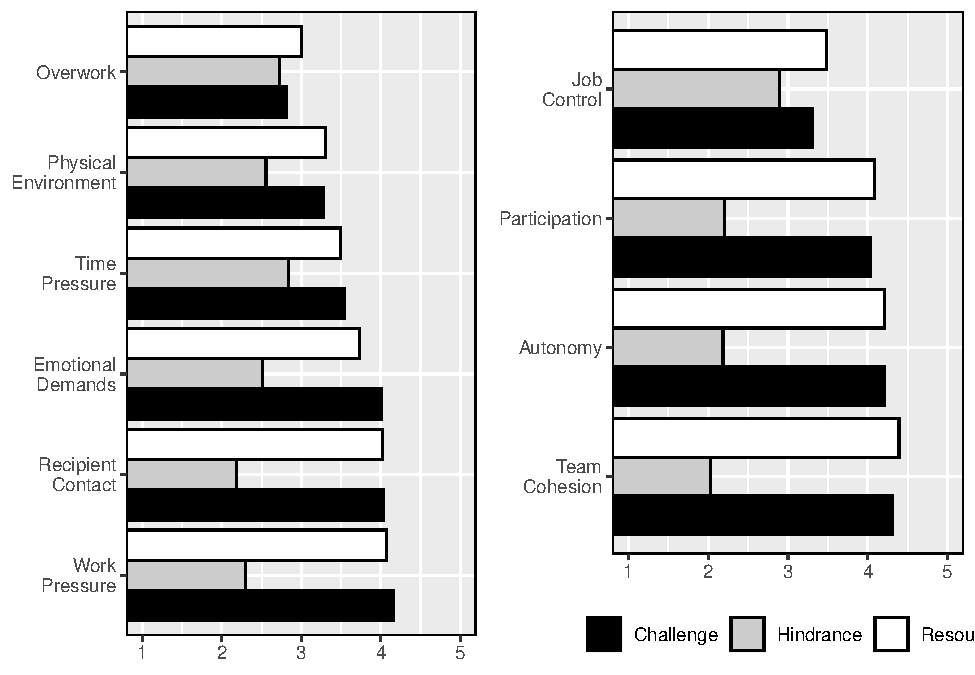
\includegraphics{Submission_files/figure-latex/scalelevelgraphs-1.pdf}
\caption{\label{fig:scalelevelgraphs}Average characteristic rating grouped by literature-implicated categorizations.}
\end{figure}

In addition to the two hypotheses, two related research questions were proposed: 1) do literature-implicated resources materialize as perceived resources and 2) do literature-implicated demands materialize as perceived demands? To answer these questions, authors first categorized O*Net items into the elements listed in the JD-R literature. For example, autonomy is frequently described as a resource. An O*Net item is, ``How much decision making freedom, without supervision, does your job offer?''. This O*Net item was retained within the ``autonomy'' category. Mean ratings of the O*Net items were then computed by element (e.g., all of the items representing autonomy) to explore whether literature-implicated resources and demands were evaluated as such.

Figure 4 presents these comparisons visually, where the bar lengths represent mean ratings within element category (e.g., the white bar represents mean O*Net resource ratings for a given JD-R element). First exploring the right side of Figure 4, there is a pattern of the highest level ratings being those of literature-derived resources (e.g., job control). As described above, the left side of Figure 4 shows literature-derived demand categories (e.g., work pressure). However, in contrast, we do not see a clear demarcation of resource and challenge, as would be expected if the job characteristics evidenced consistency (the literature-driven consistency would manifest as ``high'' gray and black bars and ``low'' white bars). In alignment with what we observed regarding variability in ratings of hindrance stressors in H1, there is much less consistency in how employees rated what should objectively be ``hindrances'' at work.

Repeated-measures ANOVAs were computed to further explain each of the patterns observed descriptively in Figure 4. The effect for Job Control was \(F_{(2, 1134)}\) = 52.78 (\(\eta^2\) = 0.08).
The effect for Participation was \(F_{(2, 1124)}\) = 991.16 (\(\eta^2\) = 0.64).
The effect for Autonomy was \(F_{(2, 1074)}\) = 951.90 (\(\eta^2\) = 0.64).
The effect for Team Cohesion was \(F_{(2, 1120)}\) = 853.39 (\(\eta^2\) = 0.60). Statistical significance was less than .001 for all four category comparisons. Here, the pattern was as expected. Across categories, resources were rated the highest (see white bars representing resources in Figure 4). However, as can be seen, mean challenge (which is a demand) was rated quite similarly and above the midpoint of 3 across JD-R categories. In fact, the means were nearly identical for resource and challenge ratings for all for categories. The literature-implied category with the lowest resource rating also has the highest hindrance rating, so job control is positive and negative.

Next, repeated-measures ANOVAs were also run for the group of literature-implicated \emph{demands} (see the left hand side of Figure 4). The effect for Overwork was \(F_{(2, 1134)}\) = 17.71 (\(\eta^2\) was 0.03). The effect for Physical Environment was \(F_{(2, 1108)}\) = 112.97 (\(\eta^2\) = 0.17). The effect for \texttt{Time\ Pressure} was \(F_{(2, 1090)}\) = 82.22 (\(\eta^2\) = 0.13). The effect for Emotional Demands was \(F_{(2, 1098)}\) = 393.43 (\(\eta^2\) = 0.42).
The effect for Recipient Contact was \(F_{(2, 1126)}\) = 1,031.73 (\(\eta^2\) = 0.65). The effect for Work Pressure was \(F_{(2, 1132)}\) = 718.12 (\(\eta^2\) = 0.56). In all cases, statistical significance was less then .001. However, the findings revealed that what the literature implicates as a demand was actually evaluated as a \emph{resource} (all resource means are above the midpoint). This is contrary to the expectation that ratings would match our assumption of what a demand constitutes. Looking at demands, there is a large difference between whether a characteristic is viewed as a challenge or hindrance. See the pattern of white resource bars on the left hand side of Figure 4. In other words, demands are viewed as resources. In sum, these results provide some support for RQ 1 and 2.

\hypertarget{discussion}{%
\section{Discussion}\label{discussion}}

The major aim and contribution of this paper was to examine whether there was variability in subjective ratings of job characteristics with respect to how much they serve as resources and demands (both challenge and hindrance), and also whether or not there is a match between the literature-implicated resources/demands and subjective ratings of these characteristics using a sample of items from O*Net. The findings broadly revealed that there was relatively more consistency in ratings of resources and challenges characteristics, and far more variability in job characteristics rated as hindrance stressors. This finding lends additional evidence to Horan et al. (2020)'s conclusion that ``\ldots stressors are only challenge or hindrance stressors to the extent that they are perceived as such by employees'' (p.~3). Lastly, we also found support for the hypothesis that job characteristics are not uniquely categorized as a resource or demand, but rather, some job characteristics are rated highly as both a resource and a demand (H2). Specifically, we consistently observed that job characteristics rated as resources were also rated viewed similarly as challenges.

\hypertarget{implications}{%
\subsection{Implications}\label{implications}}

Much of our existing research on job demands and resources has been done from the perspective that job characteristics could be classified in advance as a ``resource'' or ``demand''. Theoretically, however, our findings support a growing body of literature suggesting that perceptions of resources and demands, broadly, are not universal. There are individual differences in how employees experience the characteristics of their jobs.

These results have implications for practitioners as well, providing support for the idea that managers and supervisors can perhaps predict which characteristics are perceived as supportive to employees' performance. The reality that there are more individual difference in what employees perceive to be a hindrance and less in what is perceived to be a resource or challenge stressor is therefore in some ways encouraging. Somewhat surprisingly, hindrances are rated more variably. As such, one important implication is that of frequent communication with employees regarding their perceptions of characteristics that limit their performance. J. A. LePine et al. (2005) and Podsakoff et al. (2007) encourage organizations to incorporate strain-reducing activities like training and support to offset the negative effects of challenging job demands.

\hypertarget{limitations-and-future-directions}{%
\subsection{Limitations and Future Directions}\label{limitations-and-future-directions}}

As with all individual studies, this project was limited in scope, and as such, there are a number of avenues for future study worth exploring. First, we captured only a small number of job characteristics given the nature of our research questions. Because we asked up to four questions about each characteristic, we were limited in the number of job characteristics we could reasonably include. Related to that, we intentionally worked within the O*Net database, and in selecting job context and activity items, did not include other types of job characteristics that may be important resources/demands. For example, we included minimal ``social'' resources or interactions with one's supervisor, which the literature would suggest are important resources. Future study should explore this aspect of work. We also used the exact definitions of resource, challenge, and hindrance. It is possible that respondents did not distinguish between the challenge and resource definition as cleanly as we intended and so future research should explore this question differently. It would also be interesting to consider outcomes associated with subjective ratings.
Lastly, there may be some practical utility to pursue training interventions aimed at \emph{how} characteristics are appraised. Perhaps the clinical literature may be informative - for example, within cognitive behavioral therapeutic applications, the way in which situations are appraised can be a mechanism to help battle affective disorders such as depression.{[}\^{}check{]} Given the current findings, where the same characteristic may be viewed similarly as both a demand and resource, it is possible that framing interventions may ameliorate negative outcomes of demands such as, for example, stress or strain.

\hypertarget{conclusion}{%
\subsection{Conclusion}\label{conclusion}}

In sum, this endeavor explored the job-demands-resources literature from a unique lens, showing that there are far more individual differences in how employees perceive demands and resources than much of our current research suggests. While resources and challenges are more similarly experienced, hindrance demands show a wide amount of variability.

\newpage

\hypertarget{references}{%
\section{References}\label{references}}

\begingroup
\setlength{\parindent}{-0.5in}
\setlength{\leftskip}{0.5in}

\hypertarget{refs}{}
\begin{CSLReferences}{1}{0}
\leavevmode\vadjust pre{\hypertarget{ref-abbas2019challenge}{}}%
Abbas, M., \& Raja, U. (2019). Challenge-hindrance stressors and job outcomes: The moderating role of conscientiousness. \emph{Journal of Business and Psychology}, \emph{34}(2), 189--201.

\leavevmode\vadjust pre{\hypertarget{ref-bakker2014job}{}}%
Bakker, A. B., \& Demerouti, E. (2014). Job demands--resources theory. \emph{Wellbeing: A Complete Reference Guide}, 1--28.

\leavevmode\vadjust pre{\hypertarget{ref-bakker2017job}{}}%
Bakker, A. B., \& Demerouti, E. (2017). Job demands--resources theory: Taking stock and looking forward. \emph{Journal of Occupational Health Psychology}, \emph{22}(3), 273.

\leavevmode\vadjust pre{\hypertarget{ref-bakker2013weekly}{}}%
Bakker, A. B., \& Sanz-Vergel, A. I. (2013). Weekly work engagement and flourishing: The role of hindrance and challenge job demands. \emph{Journal of Vocational Behavior}, \emph{83}(3), 397--409.

\leavevmode\vadjust pre{\hypertarget{ref-cavanaugh2000empirical}{}}%
Cavanaugh, M. A., Boswell, W. R., Roehling, M. V., \& Boudreau, J. W. (2000). An empirical examination of self-reported work stress among US managers. \emph{Journal of Applied Psychology}, \emph{85}(1), 65.

\leavevmode\vadjust pre{\hypertarget{ref-chen2021daily}{}}%
Chen, H., Wang, H., Yuan, M., \& Xu, S. (2021). Daily challenge/hindrance demands and cognitive wellbeing: A multilevel moderated mediation model. \emph{Frontiers in Psychology}, \emph{12}, 616002.

\leavevmode\vadjust pre{\hypertarget{ref-crawford2010linking}{}}%
Crawford, E. R., LePine, J. A., \& Rich, B. L. (2010). Linking job demands and resources to employee engagement and burnout: A theoretical extension and meta-analytic test. \emph{Journal of Applied Psychology}, \emph{95}(5), 834.

\leavevmode\vadjust pre{\hypertarget{ref-demerouti2001job}{}}%
Demerouti, E., Bakker, A. B., Nachreiner, F., \& Schaufeli, W. B. (2001). The job demands-resources model of burnout. \emph{Journal of Applied Psychology}, \emph{86}(3), 499.

\leavevmode\vadjust pre{\hypertarget{ref-gerich2017relevance}{}}%
Gerich, J. (2017). The relevance of challenge and hindrance appraisals of working conditions for employees' health. \emph{International Journal of Stress Management}, \emph{24}(3), 270.

\leavevmode\vadjust pre{\hypertarget{ref-horan2020review}{}}%
Horan, K. A., Nakahara, W. H., DiStaso, M. J., \& Jex, S. M. (2020). A review of the challenge-hindrance stress model: Recent advances, expanded paradigms, and recommendations for future research. \emph{Frontiers in Psychology}, \emph{11}, 560346.

\leavevmode\vadjust pre{\hypertarget{ref-kim2020thriving}{}}%
Kim, M., \& Beehr, T. A. (2020). Thriving on demand: Challenging work results in employee flourishing through appraisals and resources. \emph{International Journal of Stress Management}, \emph{27}(2), 111.

\leavevmode\vadjust pre{\hypertarget{ref-lazarus1984stress}{}}%
Lazarus, R. S., \& Folkman, S. (1984). \emph{Stress, appraisal, and coping}. Springer publishing company.

\leavevmode\vadjust pre{\hypertarget{ref-lepine2005meta}{}}%
LePine, J. A., Podsakoff, N. P., \& LePine, M. A. (2005). A meta-analytic test of the challenge stressor--hindrance stressor framework: An explanation for inconsistent relationships among stressors and performance. \emph{Academy of Management Journal}, \emph{48}(5), 764--775.

\leavevmode\vadjust pre{\hypertarget{ref-lepine2022challenge}{}}%
LePine, M. A. (2022). The challenge-hindrance stressor framework: An integrative conceptual review and path forward. \emph{Group \& Organization Management}, \emph{47}(2), 223--254.

\leavevmode\vadjust pre{\hypertarget{ref-peterson2001understanding}{}}%
Peterson, N. G., Mumford, M. D., Borman, W. C., Jeanneret, P. R., Fleishman, E. A., Levin, K. Y., Campion, M. A., Mayfield, M. S., Morgeson, F. P., Pearlman, K., et al. (2001). Understanding work using the occupational information network (o* NET): Implications for practice and research. \emph{Personnel Psychology}, \emph{54}(2), 451--492.

\leavevmode\vadjust pre{\hypertarget{ref-podsakoff2007differential}{}}%
Podsakoff, N. P., LePine, J. A., \& LePine, M. A. (2007). Differential challenge stressor-hindrance stressor relationships with job attitudes, turnover intentions, turnover, and withdrawal behavior: A meta-analysis. \emph{Journal of Applied Psychology}, \emph{92}(2), 438.

\leavevmode\vadjust pre{\hypertarget{ref-rodell2009can}{}}%
Rodell, J. B., \& Judge, T. A. (2009). Can {``good''} stressors spark {``bad''} behaviors? The mediating role of emotions in links of challenge and hindrance stressors with citizenship and counterproductive behaviors. \emph{Journal of Applied Psychology}, \emph{94}(6), 1438.

\leavevmode\vadjust pre{\hypertarget{ref-rosen2020challenges}{}}%
Rosen, C. C., Dimotakis, N., Cole, M. S., Taylor, S. G., Simon, L. S., Smith, T. A., \& Reina, C. S. (2020). When challenges hinder: An investigation of when and how challenge stressors impact employee outcomes. \emph{Journal of Applied Psychology}, \emph{105}(10), 1181.

\leavevmode\vadjust pre{\hypertarget{ref-searle2015merits}{}}%
Searle, B. J., \& Auton, J. C. (2015). The merits of measuring challenge and hindrance appraisals. \emph{Anxiety, Stress, \& Coping}, \emph{28}(2), 121--143.

\leavevmode\vadjust pre{\hypertarget{ref-selye1936syndrome}{}}%
Selye, H. (1936). A syndrome produced by diverse nocuous agents. \emph{Nature}, \emph{138}(3479), 32--32.

\leavevmode\vadjust pre{\hypertarget{ref-webster2010toward}{}}%
Webster, J. R., Beehr, T. A., \& Christiansen, N. D. (2010). Toward a better understanding of the effects of hindrance and challenge stressors on work behavior. \emph{Journal of Vocational Behavior}, \emph{76}(1), 68--77.

\leavevmode\vadjust pre{\hypertarget{ref-webster2011extending}{}}%
Webster, J. R., Beehr, T. A., \& Love, K. (2011). Extending the challenge-hindrance model of occupational stress: The role of appraisal. \emph{Journal of Vocational Behavior}, \emph{79}(2), 505--516.

\leavevmode\vadjust pre{\hypertarget{ref-R-careless}{}}%
Yentes, R. D., \& Wilhelm, F. (2021). \emph{Careless: Procedures for computing indices of careless responding}.

\end{CSLReferences}

\endgroup


\end{document}
